% preamble
\documentclass[twoside]{report}

% importing packagess
\usepackage[english]{babel}
\usepackage[utf8]{inputenc}

\usepackage{graphicx}
\graphicspath{{images/}}

\usepackage{caption}
\usepackage{subcaption}

% \usepackage[top=1in, bottom=1in, bindingoffset=1.5in]{geometry}
\usepackage[a4paper,width=150mm,top=25mm,bottom=25mm, bindingoffset=6mm]{geometry}
\usepackage{fancyhdr}
\usepackage{blindtext}

\newcommand{\serviceName}{Phineas}


% \usepackage{hyperref}
% what does this do?
\pagestyle{fancy}


% clear out heading settings
\fancyhead{}

% on the Right side of Odd pages, put PDD
% on the Left side of Even pages, put PDD
\fancyhead[RO, LE]{\serviceName Design Document}

\fancyfoot{}
\fancyfoot[LE, RO]{\thepage}
\fancyfoot[LO, CE]{Chapter \thechapter}
\fancyfoot[CO, RE]{Steeve Joseph}




% end preamble

\title{\serviceName\ Software Design Document}
\author{Steeve Joseph}
\date{7 December 2019}

\begin{document}
\maketitle
\tableofcontents
\listoffigures
\listoftables


% importing Introduction.tex's content to be the content of the chapter
\chapter{Introduction}
\section{Purpose}
Currently, with creative fields being as saturated as they are, 
it is difficult for a newcomer into the "service arts", such as photography, commision painting, and singing,
to find clientele. The typical creative has difficulty marketing their services, and this is likely because 
their services are not being marketed "properly". In agile software development, there is an emphasis on 
finding a demographic of people to solve a problem for, and then developing a product that acts as a solution
to that problem. With this methodology, the organization developing the product has sought out and matched their target clientele.

However, in more "creative-oriented" fields, this does not seem to be the representative approach. The default approach from the 
creative seems to be to cast a wide net so to speak, and hopefully net some buyers.

If it were possible to filter/pre-select potential clients on some objective and/or measurable metric, the artist 
would presumably have higher success pitching themselves the clients with whom they "match".

\section{Scope}
The scope of this project thus far is to be used as a photographer looking for likely candidates for clientele,
using social media. Specifically, the product would allow a photographer to single out people that are interested in the genres that the 
photographer is seeking to shoot, based on hashtags, thereby facilitating the filtering process for the photographer.

\section{Overview}
A representative use-case for the product is given below:

1. The user signs into \serviceName with their Instagram account.

2. The user searches hashtags matching what they want to take pictures of.

3. The user gets a curated list of potential clients that they can then contact.

\section{Reference Material}
\section{Definitions and Acronyms}
\begin{table}[ht]
    \centering
    \begin{tabular}{l | l}
        Term & Definition \\
        \hline
        IG & Instagram \\
        FB & Facebook \\
        IGAPI & Instagram Platform API \\
        FBGA & Facebook Graph API \\
        FBBDA & Facebook Basic Display API \\
        MVP & Minimum Viable Product \\
    \end{tabular}
    \caption{Table of Definitions and acronyms used}
    \label{tab: def_ac}
\end{table}



% \blindtext[6]

\chapter{System Overview}
\input{chapters/2-SystemOverview.tex}

\chapter{System Architecture}
\section{Design Constraints}

\subsection{Instragram Platform API}
\subsubsection{Deprecation}
As originally anticipated, the Basic display portion of the IG Platform API was set to be deprecated by early 2020,
accelerating the timeline for this project significantly. Essentially, the intent was to get a working prototype/
minimum viable product (MVP) released before deprecation. Of course, deprecation would still have to be accounted for,
but the benefits of the MVP could have been reaped in the meantime. A potentially unaccounted for change is the effect 
of the deprecation of the Public Content endpoints on the ability to query for images based on hashtags.
This is mentioned because it is a critical feature of \serviceName.

\subsubsection{Discontinuation of New Client Registration}
An unanticipated hiccup was the discontinuation of new client registrations by the IG Platform,
essentially forcing the use of the Instagram Graph API. This was retroactively discovered after the discontinuation
in \date{October 15, 2019}.

% @steeve: look into details of Graph API
\subsection{Instagram Graph API}
The Instagram Graph API is the successor to the Instagram Platform API (sometimes referred to as the Legacy API)
Presumably, this API implements GraphQL in order to limit the amount of data sent with each request.

The benefit of this is better control of privacy issues across the platform. The potential drawback is that
the Graph API may not have the full functionality that the IG Platform API had, for good reason as well.
Facebook seems to be moving in a direction wherein the level of user information is limited, most likely to mitigate potential harm from bad actors.


\subsubsection{Limitations}
The critical functionality of \serviceName is using Instagram's API to gather a set of pictures based on hashtags,
and filter for users that meet a certain set of requirements. These requirements are predicated on metrics such as:
user follower count, user following count, likes on said picture, comments on said picture, etc. It seems that 
the Graph API is solely concerned with business accounts, as of \date{\today}, and that regular personal accounts
do not have public API endpoints exposed. The following are points of interest in the new API.

\subsubsection{IG User Endpoints}
Represents an Instagram Business Account or an Instagram Creator Account. Some relevant returnable fields from
this endpoint are:
\begin{itemize}
    \item biography
    \item followers\_count
    \item follows\_count
    \item name
    \item username
    \item website
\end{itemize}

Relevant edges are:
\begin{itemize}
    \item Business Discovery: Allows you to get data about other Instagram Business or Creator IG Users.
    \item Insights: Represents social interaction metrics on an IG User. 
    \item Media
    \item Recently Searched Hashtags
\end{itemize}


\subsubsection{IG User: Insights}

\subsubsection{IG Media}
Represents and Instagram photo, video, story, or album.

Relevant returnable fields from this object are:
\begin{itemize}
    \item caption
    \item children (if IG album)
    \item comments
    \item comments\_count
    \item like\_count
    \item permalink
    \item username
    \item media\_type
    \item timestamp
\end{itemize}

\subsubsection{IG Media: Insights}
Represents social interaction metrics on an IG Media object. Relevant metrics include 
\begin{itemize}
    \item Photo and Video Metrics
    \begin{itemize}
        \item engagement: Total number of likes and IG Comments on the album IG Media object.
        \item impressions: Total number of times the album IG Media object has been seen.
        \item reach: Total number of unique Instagram accounts that have seen the album IG Media object.
        \item saved: Total number of unique Instagram accounts that have saved the album IG Media object.
        \item video\_views
    \end{itemize}

    \item Album Metrics
    \begin{itemize}
        \item carousel\_album\_engagement: Total number of likes and IG Comments on the album IG Media object.
        
        \item carousel\_album\_impressions: Total number of times the album IG Media object has been seen.
        
        \item carousel\_album\_reach: Total number of unique Instagram accounts that have seen the album IG Media object.
        
        \item carousel\_album\_saved: Total number of unique Instagram accounts that have saved the album IG Media object.
    \end{itemize}
    \item Story Metrics
    \begin{itemize}
        \item exits: Number of times someone exited the story IG Media object.
        
        \item  impressions: Total number of times the story IG Media object has been seen.
        
        \item reach: Total number of unique Instagram accounts that have seen the story IG Media object.
        
        \item replies: Total number of replies (IG Comments) on the story IG Media object.
        
        \item  taps\_forward: Total number of taps to see this story IG Media object's next photo or video.

        \item taps\_back: Total number of taps to see this story IG Media object's previous photo or video.
    \end{itemize}
\end{itemize}


\subsubsection{IG Hashtag}
Represents an Instagram hashtag. Relevant edges from this node are
\begin{itemize}
    \item \textbf{Recent Media} Returns a collection of media recently tagged with this hashtag.
    \item \textbf{Top Media} Returns a collection of the most popular media tagged with this hashtag.
\end{itemize}

\subsubsection{IG Hashtag: Recent Media}
Represents a collection of the most recently published photo and video IG Media objects that have been tagged with a hashtag.

\subsubsection{Comments}
Represents a collection of IG Comments on an IG Media object. Not readily apparent what value these have,
may be possible to perform aggregate sentiment analysis on an IG Media Object's comments.

\subsection{Instagram Basic Display API}
The Instagram Basic Display API seems to replicate the functionality of the Legacy API's Basic panel, 
which allowed the reading a user's profile info and media. While there is a plethora of useful information accessable,
some core components that seem to be missing are:
\begin{itemize}
    \item user follower count
    \item user following count
    \item user engagement metrics
\end{itemize}
The lack of the above fields indicate Instagram's focus on privacy and security for regular accounts.
As a result, \serviceName will be primarily focused on Creator and Business Instagram accounts,
which have more information readilt available.
\subsubsection{Limitations}
\section{Prior Attempts}
This section focuses on prior attempts at solving the problem mentioned in the Introduction. 

\section{Similar Software}
To date, (\date{\today}), there does not seem to be any similar products or services in this space.
Specifically, many of the applications using Instagram's API are using the Legacy version, either from presumable reluctance
to migrate, or due to perceived lack of functionality in the Graph and Basic Display APIs.

\chapter{Data Design}
\section{Database Design}
MongoDB will be used for \serviceName, using MongoDB Atlas as the database provider.

The databse currently looks like this:
\begin{figure}[ht]
    \centering
    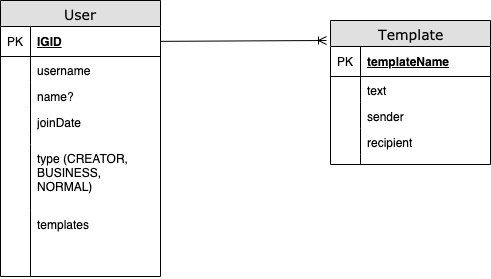
\includegraphics[scale=0.5]{phind_ERD.png}
    \caption{Phind ERD}
    \label{}
\end{figure}

\section{User Model}
The User model will look like this:

\begin{figure}[ht]
    \centering
    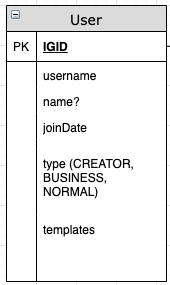
\includegraphics[scale=0.5]{phind_user_model.png}
    \caption{Phind user model}
    \label{find use}
\end{figure}

\section{Data Interaction}
\serviceName will read and write to a MongoDB database via an API written in ExpressJS. The API will communicate
with a ReactJS frontend.

\chapter{Component Design}
\section{API}
This section covers implementation details for the API of this service.

\subsection{Backend Language}
ExpressJS was chosen to be the backend language of choice for this service.  The reasons why are numerous:
\begin{itemize}
    \item written in JS
    \item simple, flexible, extensible
    \item "One language to rule them all"
\end{itemize}

\subsection{Routes}
At the very least, the necessary routes are:
\begin{itemize}
    \item login: goes through Instagram's auth flow
    \item query: takes in a query object, returns a list of users
\end{itemize}


\section{User Interface}
This section covers implementation details of the UI portion of this service. This service will primarily be web-based. ReactJS will be used as the UI framework. Rationale:
\begin{itemize}
    \item It is the framework I know best
    \item Fits into "one language to rule them all" paradigm
\end{itemize}


\chapter{User Interface Design}
\section{UI Overview}
\section{Screenshots}
\section{Screen Objects and Actions}


\chapter{Requirements}
\input{chapters/7-Requirements.tex}

\chapter{Milestones}
\input{chapters/8-Milestones.tex}

\chapter{Testing}
\section{API Testing}
\subsection{Postman}
\subsubsection{Collections}
A collection is used to run multiple requests (and their coresponding tests) simultaneouslty
\subsubsection{Tests}
In addition, fields from the response of one request can be used in another request via chaining.

\section{GUI Testing}
\subsection{Selenium}
\subsection{Squish Tools}


\end{document}